\documentclass{article}
\usepackage{graphicx} % Required for inserting images
\usepackage{amsmath} % For mathematical formatting
\DeclareMathOperator*{\lcm}{lcm}
\usepackage{amsthm} % For theorem environments
\usepackage{amssymb} % For \blacksquare
\usepackage{xparse}
\usepackage{tikz} % for squares
\usepackage{yfonts}
\usepackage{changepage}

\title{Theorems, definitions and corollaries\\ for Modern Algebra}
\author{Marco Antonio Peña Ibarra}
\date{}

\begin{document}
\maketitle

\section*{$\bigstar$ Week 2}
\section*{GROUPS!}
\textbf{Definition:} Given a set \(G\), we impose a few definitions on it.
\begin{enumerate}
    \item A binary operation \(\star\) on a set \(G\) is a function 
    \[\star:G\star G \xrightarrow{}G\]
    For any \(a,b\in G\) we have \(a\star b \in G\).
    \item \(\star\) is associative on \(G\) if \(\forall a,b,c \in G\)
    \[a \star (b \star c)=(a \star b)\star c\]
    \item If for every \(a,b \in G\), \(a \star b=b \star a\), then \(\star\) (and hence \(G\)) is commutative (or abelian).\\[0.5cm]
\end{enumerate}

\flushleft{\textbf{Definition:}} A \textbf{group} is an ordered pair \((G,\star)\) where \(G\) is a set and \(\star\) is a binary operation on \(G\) such that:
\begin{enumerate}
    \item \textbf{Closure:} For any two elements \(a,b \in G\), the result of the operation \(a \star b\) must be also in \(G\).
    \item \textbf{Associativity:} \(\star\) is associative.
    \item \textbf{Identity:} There exists an element \(e\in G\) called the identity of \(G\) under \(\star\) such that \(\forall a \in G\), \[a \star e=e\star a=a\] and \(e\) commutes with all the elements of \(G\).
    \item \textbf{Inverse:} For any \(a\in G\), there exists \(a^-1\) an element such that \[a\star a^-1=a^1 \star a=e\]\\
\end{enumerate}

\centerline{\textbf{Examples of a group}}
\begin{enumerate}
    \item[] Integers under addition \((\mathbb{Z},+)\)
    \item[] Real numbers under addition \((\mathbb{R},+)\)
    \item[] Non-zero real numbers under multiplication \((\mathbb{R^*}, \times)\)
\end{enumerate}

\centerline{\textbf{Examples of what is NOT a group}}
\begin{enumerate}
    \item[] Why isn't \((\mathbb{Z}\setminus\{0\},\times)\) a group? Because there are not inverses for every element.
    \[a\times a^{-1}=1\]
    \[2 \times \frac{1}{2}=1\]
    But notice that \(\frac{1}{2}\) is not an integer.\\[1cm]

\end{enumerate}


\textbf{Proposition:} Let \((G, \star)\) be a group. Then
\begin{enumerate}
    \item \(e \in G\) is unique
    \item For each \(a \in G\), the inverse \(a^{-1}\) is uniquely determined
    \item \((a^{-1})^{-1}=a\) for all \(a \in G\)
    \item \((a \star b)^{-1}=b^{-1}\star a^{-1}\)
\end{enumerate}
\clearpage

\section*{$\bigstar$ Week 3}
\section*{Dihedral and Symmetrical Groups!}

\textbf{Definition:} Let \(G\) be a group with \(x \in G\).\\
We say that the \textbf{order} of \(x\) is the smallest positive integer \(n\) such that
\[x^n=1\]
We denote the order of \(x\) by \(|x|\) and say that \(x\) is of order \(n\)
\[|x|=n\]
If there is NO positive integer \(n\) for a given \(x\), then we say that \(x\) has infinite order.\\[0.5cm]

\centerline{\textbf{Examples of orders:}}
What can be said if \(|a|=1?\) Then \(a=e\),\\if \(|a|=2?\) Then, \(a=a^{-1}\)\\[0.3cm]

Consider \(G=(\mathbb{Z}/8\mathbb{Z}, +)\). The set of residues modulo 8 under addition
\begin{align*}
|0|&=1\\
|1|&=8\\
|2|&=4\\
|3|&=8\\
|4|&=2\\
|5|&=8\\
|6|&=4\\
|7|&=8\\
\end{align*}

{\textbf{Definition:}} A \textbf{dihedral group} is the group of symmetries of a regular polygon, which includes both rotations and reflections.\\[0.2cm]
\textit{Note:} Dihedral groups are an essential class of abstract algebra groups that arise naturally in geometry and other areas of mathematics.
\(D_{2n}\) means the dihedral group on \(n\) vertices or elements.\\[0.5cm]
\centerline{\textbf{Notation for the Dihedral Group}}
\begin{enumerate}
    \item[] \(r\): clockwise rotation about the origin (center) by \(2\pi/n \) radians.
    \item[] \(s\): reflection/flip
\end{enumerate}

\newpage
\textbf{Definition:} \(r\) and \(s\) are the \textbf{generators} of \(D_{2n}\) if
\[D_{2n}=<r,s \mid r^n=s^2=1, rs=sr^{-1}>\]
Here, \(r,s\) represent the generators of \(D_{2n}\) and \(r^n=s^2=1, rs=sr^{-1}\) the \textbf{relations} of the generators.\\[0.5cm]

\centerline{\textbf{Example of the table of a group}}
What group is this?
\[<x,y \mid x^2 = y^2 = (xy)^2 =1>\]
Make a multiplication table [Cayley tables]
\begin{table}[h]
    \centering
    \begin{tabular}{c|ccccc}
        $G$ & 1 & $x$ & $y$ & $xy$ \\
        \hline
        1 & 1 & $x$ & $y$ & $xy$ \\
        $x$ & $x$ & 1 & $xy$ & $y$ \\
        $y$ & $y$ & $yx$ & 1 & $x$ \\
        $xy$ & $xy$ & $y$ & $x$ & 1 \\
    \end{tabular}
    \caption{Group Operation Table}
    \label{tab:group_operation}
\end{table}\\

\flushleft{\textbf{Definition:} \underline{Well defined:} unambigous}\\
Let \(G=\{x \in \mathbb{R} \mid 0 \leq 0 < 1\}\), where \(x \neq y\) is the \textbf{fractional part} of \(x+y\).
\begin{center}
    i.e. \(x \star y=x+y-[x+y]\)\\
    where \([a]\) is the greatest integer less than or equal than \(a\).\\
    ex. \(\pi \star e= 3.14...+2.71...-[3+2]\)\\[0.5cm]
\end{center}

\textbf{Definition:} Symmetrical Groups
\begin{itemize}
    \item Let \(S_\Omega\) (where \(\Omega\) is a non empty set) is the set of all bijections from \(\Omega\) to itself [all permutations are non riged symmetries].
    \item \(S_\Omega\) is a group under function composition and is called the symmetric group on \(|\Omega|=n\) elements.
    \item The elements in \(S_\Omega\) are permutations of the elements in \(\Omega\). [usually we have \(S_n\) for a natural number \(n\).]\\
\end{itemize}

\centerline{\textbf{Example of permutations}}
\begin{itemize}
    \item \(|S_n|=n!\)
    \item \(S_3\). Compute all the permutations of \(\{a,b,c\}\). \begin{center}
        \(|S_3|=3!=6\)\\
        6 possible permutations on a set of 3 elements.
    \end{center}
\end{itemize}

\textbf{Definition:} Cycle decomposition [\(\sigma \in S_n\)]\\
A \textbf{cycle} is a string of integers which represents the elements of \(S_n\) which cyclically permutes these integers and fixes all others.\\
\begin{itemize}
    \item The cycle \((1\ 2\ 3\ 4)\) reads like this: \begin{center}
        1 gets sent to 2\\
        2 gets sent to 3\\
        3 gets sent to 4\\
        4 gets sent to 1\\
    \end{center}

    \begin{center}
\begin{tikzpicture}
    % First square
    \draw (0,0) rectangle (2,2); 
    \node[anchor=south west] at (0,2) {1}; 
    \node[anchor=south east] at (2,2) {2}; 
    \node[anchor=north east] at (2,0) {3}; 
    \node[anchor=north west] at (0,0) {4}; 
    
    % Second square (shifted to the right)
    \draw (3,0) rectangle (5,2);
    \node[anchor=south west] at (3,2) {4}; 
    \node[anchor=south east] at (5,2) {1}; 
    \node[anchor=north east] at (5,0) {2}; 
    \node[anchor=north west] at (3,0) {3}; 
\end{tikzpicture}
    \end{center}

    \item The cycle \((2\ 4\ 1\ 3)\) reads like this: \begin{center}
        2 gets sent to 4\\
        4 gets sent to 1\\
        1 gets sent to 3\\
        3 gets sent to 2\\
    \end{center}

    \begin{center}
\begin{tikzpicture}
    % First square
    \draw (0,0) rectangle (2,2); 
    \node[anchor=south west] at (0,2) {1}; 
    \node[anchor=south east] at (2,2) {2}; 
    \node[anchor=north east] at (2,0) {3}; 
    \node[anchor=north west] at (0,0) {4}; 
    
    % Second square (shifted to the right)
    \draw (3,0) rectangle (5,2);
    \node[anchor=south west] at (3,2) {4}; 
    \node[anchor=south east] at (5,2) {3}; 
    \node[anchor=north east] at (5,0) {1}; 
    \node[anchor=north west] at (3,0) {2}; 
\end{tikzpicture}
    \end{center}
\end{itemize}

\newpage
\centerline{\textbf{Example of a cycle decomposition}}
Let \(n=13\) and \(\sigma \in S_{13}\) be defined by
\begin{align*}
    \sigma(1)&=12\\
    \sigma(2)&=13\\
    \sigma(3)&=3\\
    \sigma(4)&=1\\
    \sigma(5)&=11\\
    \sigma(6)&=9\\
    \sigma(7)&=5\\
    \sigma(8)&=10\\
    \sigma(9)&=6\\
    \sigma(10)&=4\\
    \sigma(11)&=7\\
    \sigma(12)&=8\\
    \sigma(13)&=2\\
\end{align*}
So, \(\sigma=(1\ 12\ 8\ 10\ 4)(2\ 13)(3)(5\ 11\ 7)(6\ 9)\)\\
\underline{Fact:} \(\sigma \sigma^{-1}=e\)\\

\newpage
\section*{$\bigstar$ Week 4}
\section*{Homomorphisms and Isomorphisms, Group Actions!}

\textit{Note:} Monoid \(\subseteq\) Groups \(\subseteq\) Rings \(\subseteq\) Fields\\

\flushleft{\textbf{Definition:}} A \textbf{field} is the "smallest" mathematical structure in which we can do arithmetic: \(+, -, \times,/\) as usual.\\[0.5cm]

\centerline{\textbf{Example of what is a field}}
\begin{align*}
    \mathbb{Q} &-\text{Rational numbers}\\
    \mathbb{R} &-\text{Real numbers}\\
    \mathbb{Z}/5\mathbb{Z} &-\{0,1,2,3,4\}
\end{align*}\\[0.5cm]

\flushleft{\textbf{Notation:}} The Quaternion Group\\
Implies number: \(\{1,-1,i,-i\}\)\\
\begin{table}[h]
    \centering
    \begin{tabular}{c|c|c|c|c|c}
        $x$ & 1 & $i$ & $j$ & $k$ \\
        \hline
        1 & 1 & $i$ & $j$ & $k$ \\
        $i$ & $i$ & -1 & $ij=k$ & $ik=-j$ \\
        $j$ & $j$ & $ji=-k$ & -1 & $jk=-i$ \\
        $k$ & $k$ & $ki=j$ & $kj=-i$ & -1 \\
    \end{tabular}
    \caption{Quaternion Multiplication Table}
    \label{tab:group_operation}
\end{table}

\flushleft{\textbf{Definition:}} Homomorphisms and Isomorphisms\\
Let \(G,H\) be groups.\\
A map \(\phi:G \xrightarrow{}H\) is called a \textbf{homomorphism}.\\
If for every \(a,b \in G\), \[\phi(ab)=\phi(a)\phi(b)\] where \(\phi(ab) \xrightarrow{}\) operations in \(G\) and \(\phi(a)\phi(b) \xrightarrow{}\) operations in \(H\).\\[0.5cm]

\newpage
For all \(a,b \in G\)


\begin{center}
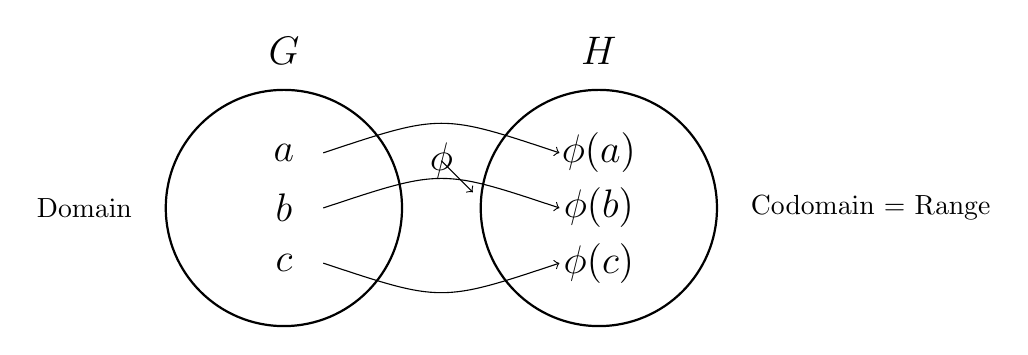
\begin{tikzpicture}

    % Draw the domain circle
    \draw[thick] (-2,0) circle (1.5) node[left=1.8cm] {Domain};

    % Draw the codomain circle
    \draw[thick] (2,0) circle (1.5) node[right=1.8cm] {Codomain = Range};

    % Labels for sets G and H
    \node at (-2,2) {\Large $G$};
    \node at (2,2) {\Large $H$};

    % Elements inside the domain
    \node at (-2,0.7) {\Large $a$};
    \node at (-2,0) {\Large $b$};
    \node at (-2,-0.7) {\Large $c$};

    % Elements inside the codomain
    \node at (2,0.7) {\Large $\phi(a)$};
    \node at (2,0) {\Large $\phi(b)$};
    \node at (2,-0.7) {\Large $\phi(c)$};

    % Mapping arrows
    \draw[->] (-1.5,0.7) .. controls (0,1.2) .. (1.5,0.7);
    \draw[->] (-1.5,0) .. controls (0,0.5) .. (1.5,0);
    \draw[->] (-1.5,-0.7) .. controls (0,-1.2) .. (1.5,-0.7);

    % Function notation
    \node at (0,0.6) {\Large $\phi$};
    \draw[->] (0,0.6) -- (0.4,0.2);

\end{tikzpicture}
\end{center}

A map from a group to another is a homomorphism if the map preserves the group structures of its domain in the codomain (range).\\[0.5cm]

\flushleft{\textbf{Definition:}} The map \(\phi:G \xrightarrow{}H\) (where \(G\) and \(H\) are groups) is called an \textbf{isomomorphism} and \(G\) and \(H\) are said to be isomorphic.\\
\(G \cong H\) if
\begin{enumerate}
    \item \(\phi\) is a homomorphism
    \item \(\phi\) is a bijection (find the inverse" \(\phi^{-1}\))
\end{enumerate}
In other words, \(G\) and \(H\) are identical up to the "the letters on the page" \(\phi^{-1}\phi(x)=x\)\\[0.5cm]

\centerline{\textbf{Example of an isomorphism}}
\(\exp:\mathbb{R} \xrightarrow{} \mathbb{R}^+\) defined by \(\exp(x)=e^x\) is an isomorphism from \((\mathbb{R},+)\) to \((\mathbb{R^+},\times)\).
\begin{itemize}
    \item \(\exp\) is a bijection: \(log(\exp(x))=x\)
    \item \(\exp\) preserves operation: \(\exp(a+b)=e^ae^b=e^{a+b}=\exp(a)\exp(b)\)\\[0.5cm]
\end{itemize}

\flushleft{\textbf{Definition:}} Group actions: groups acting on sets\\
\(\bigstar \text{Big idea} \bigstar \xrightarrow{}\) A tool for taking groups apart!\\
A \textbf{group action} of a group \(G\) on a set \(A\) is a map from \(G \times A \xrightarrow{} A\) [which we can write as \(ga\), for all \(g \in G\) and \(a \in A\)] satisfying the following properties:
\begin{enumerate}
    \item \(g_1(g_2a)=(g_1g_2)(a)\), \(\forall g_1,g_2 \in G \text{ and  } a \in A\)
    \item \(1a=a\), \(\forall a \in A\)
\end{enumerate}
The expression \(ga\) does not have a binary operation. The expression is a group operation where \(ga\) is an element in \(A\).
\begin{center}
    \(f(x)=y\)\\
    \(f:\mathbb{R} \xrightarrow{} \mathbb{R}\)\\
    \(f \times \mathbb{R}\) \(\xrightarrow{} \mathbb{R}\)
\end{center}

\newpage
Observations on the definition of group action \(\star\)
\begin{itemize}
    \item Let the group \(G\) act on the set \(A\).\\
    For each fixed \(g \in G\), we get a map \(\sigma_g\) defined by \begin{center}
        \(\sigma_g: A \xrightarrow{} A\)\\
        \(\sigma_g(a)=ga\)
    \end{center}

    \item A group action of \(G\) on a set \(A\) means that every element \(g \in G\) \underline{acts} as a permutation on \(A\) consistent with the group operation in \(G\).\\ 2 FACTS! \begin{enumerate}
        \item[i)] For each fixed \(g \in G\), \(\sigma_g\) is a permutation of \(A\).
        \item[ii)] The map from \(G\) to \(S_A\) defined by \(g \mapsto \sigma_g\) is a homomorphism.
    \end{enumerate}
\end{itemize}

\newpage
\section*{$\bigstar$ Week 5}
\section*{SUBGROUPS!}

\vspace{0.5cm}
\flushleft{\textbf{Definition:}} The center of a group\\
We define \[Z(G)=\{g \in G \mid gx=xg ,\hspace{0.5cm} \forall x \in G\}\]
The center of \(G\) is the set of elements of \(G\) that commute with every element of \(G\).\\
\textit{Note:} \(Z(G)=C_G(G)\)


\vspace{0.5cm}
\flushleft{\textbf{Definition:}} Centralizer\\
Let \(G\) be a group and \(A\) be any non empty subset of the group \(G\). The centralizer is denoted as:
\[C_G(A)=\{g \in G \mid gag^{-1}=a, \hspace{0.5cm} \forall a \in A\}\]
The \underline{centralizer} is the set of elements of \(G\) that commute with every element of \(A\).
\[gag^{-1}=a \iff ga=ag\]

\vspace{0.5cm}
\flushleft{\textbf{Definition:}} Normalizer\\
The \underline{normalizer} of a set \(A\) in the group \(G\) is the set of all elements in the group that commute with the elements of \(A\).
\[N_G(A)=\{g \in G \mid gAg^{-1}=A\}\]
\textit{Note:} If \(g \in C_G(A)\), then \(gag^{-1}=a\) for all \(a \in A)\) and so \(C_G(A) \leq N_G(A)\)
    
    \vspace{0.5cm}
    \centerline{\textbf{Examples:}}
    \begin{adjustwidth}{40pt}{40pt}
        If \(G\) is abelian, then
        \[Z(G)=C_G(A)=N_G(A)=G\]
        for any subset \(A\) in \(G\).
    \end{adjustwidth}


\newpage
\section*{$\bigstar$ Week 6}
\section*{Cyclic subgroups!}
\vspace{0.5cm}
\flushleft{\textbf{Definition:}} Cyclic groups and cyclic subgroups\\
A group \(H\) is \underline{cyclic} if \(H\) can be generated by a single element from \(H\).
\[H=\{x^n \mid n \in \mathbb{Z}\} \hspace{0.5cm} H=\langle x, \times \rangle\]
\[H=\{ nx \mid n \in \mathbb{Z} \} \hspace{0.5cm} H=\langle x, + \rangle\]

\textit{Facts:}\\
A cyclic group is generated by one element.\\
\(D_8\) is not cyclic. \(S_n\) is not cyclic for any \(n\).\\
\(\mathbb{Z}/p\mathbb{Z}\) is cyclic (under addition).\\
Cyclic groups are abelian.

\vspace{0.5cm}
\flushleft{\textbf{Theorem:}}
Cyclic groups of the same order are isomorphic.

\vspace{0.5cm}
\flushleft{\textbf{Notation:}} \(Z_n\) is a cyclic group of order \(n\).
\[Z_n \cong \mathbb{Z}/n \mathbb{Z}\]

\newpage
\section*{$\bigstar$ Week 8}
\section*{Quotient groups and homomorphisms!}

\flushleft{\textbf{Definition:}} Kernel\\
If \(\phi\) is a homomorphism \(\phi : G \xrightarrow{}H\) we define the kernel of \(\phi\) to be the set
\[\{g \in G \mid \phi (g)=e=id\} \hspace{0.5cm} e=1=0\]
and is denoted by \(ker(\phi)\) where \(e\) is the \(id\) in \(H\).

\vspace{0.5cm}
\flushleft{\textbf{Proposition:}}
Let \(G,H\) be groups and let \(\phi : G \xrightarrow{}H\) be homomorphism.
\begin{enumerate}
    \item[1)] \(\phi(1_G)=1_H\) where \(1_G\) and \(1_H\) are the identity in \(G\) and \(H\).
    \item[2)] \(\phi(g^{-1})=(\phi(g))^{-1} \hspace{0.5cm} \forall g \in G\)
    \item[3)] \(\phi(g^n)=(\phi(g))^n \hspace{0.5cm} \forall n \in \mathbb{Z}\)
    \item[4)]  \(Ker(\phi) \leq G\)
    \item[5)] \(im(\phi) \leq H\) where \(im(\phi)\) is the image of \(G\) under \(\phi\).
\end{enumerate}


\end{document}
